%%%%%%%%%%%%%%%%%%%%%%%%%%%%%%%%%%%%%%%%%
% Structured General Purpose Assignment
% LaTeX Template
%
% This template has been downloaded from:
% http://www.latextemplates.com
%
% Original author:
% Ted Pavlic (http://www.tedpavlic.com)
%
% Note:
% The \lipsum[#] commands throughout this template generate dummy text
% to fill the template out. These commands should all be removed when 
% writing assignment content.
%
%%%%%%%%%%%%%%%%%%%%%%%%%%%%%%%%%%%%%%%%%

\documentclass{article}

\usepackage{fancyhdr} % Required for custom headers
\usepackage{lastpage} % Required to determine the last page for the footer
\usepackage{extramarks} % Required for headers and footers
\usepackage{graphicx} % Required to insert images
\usepackage[latin1]{inputenc}

% Margins
\topmargin=-0.45in
\evensidemargin=0in
\oddsidemargin=0in
\textwidth=6.5in
\textheight=9.0in
\headsep=0.25in 

\linespread{1.1} % Line spacing



\setlength\parindent{0pt} % Removes all indentation from paragraphs

%----------------------------------------------------------------------------------------
%	DOCUMENT STRUCTURE COMMANDS
%	Skip this unless you know what you're doing
%----------------------------------------------------------------------------------------

% Header and footer for when a page split occurs within a problem environment
\newcommand{\enterProblemHeader}[1]{
\nobreak\extramarks{#1}{#1 continued on next page\ldots}\nobreak
\nobreak\extramarks{#1 (continued)}{#1 continued on next page\ldots}\nobreak
}

% Header and footer for when a page split occurs between problem environments
\newcommand{\exitProblemHeader}[1]{
\nobreak\extramarks{#1 (continued)}{#1 continued on next page\ldots}\nobreak
\nobreak\extramarks{#1}{}\nobreak
}

\setcounter{secnumdepth}{0} % Removes default section numbers
\newcounter{homeworkProblemCounter} % Creates a counter to keep track of the number of problems
%----------------------------------------------------------------------------------------
%	NAME AND CLASS SECTION
%----------------------------------------------------------------------------------------

\newcommand{\lessonNumber}[1]{Lezione\ \##1} % Assignment title
\newcommand{\lessonDate}[4]{#1,\ #2\ #3\ #4} % Due date
\newcommand{\lessonCourse}[1]{#1} % Course/class
\newcommand{\lessonTime}[1]{#1} % Class/lecture time
\newcommand{\lessonTeacher}[1]{#1} % Teacher/lecturer
\newcommand{\lessonAuthor}[1]{#1} % Your name

% Set up the header and footer
\pagestyle{fancy}
\lhead{\lessonAuthor{Luca De Franceschi}} % Top left header
\chead{\lessonAuthor{Tullio Vardanega}\ \lessonTime{9:30}: \lessonNumber{18}} % Top center header
\rhead{\firstxmark} % Top right header
\lfoot{\lastxmark} % Bottom left footer
\cfoot{} % Bottom center footer
\rfoot{Page\ \thepage\ of\ \pageref{LastPage}} % Bottom right footer
\renewcommand\headrulewidth{0.4pt} % Size of the header rule
\renewcommand\footrulewidth{0.4pt} % Size of the footer rule

%----------------------------------------------------------------------------------------
%	TITLE PAGE
%----------------------------------------------------------------------------------------

\title{
\vspace{2in}
\textmd{\textbf{\lessonNumber{18}}\\
\normalsize\vspace{0.1in}\small{\lessonDate{Marted�}{19}{Novembre}{2013}}\\
\vspace{0.1in}\large{\textit{\lessonTeacher{Tullio Vardanega},\ \lessonTime{9:30-11:30}}}
\vspace{3in}
}
}

\author{\textbf{\lessonAuthor{Luca De Franceschi}}}
\date{} % Insert date here if you want it to appear below your name

%----------------------------------------------------------------------------------------

\begin{document}

\maketitle
\newpage
\newpage

\textbf{Progettazione Software}\\\\

Progettare prima di produrre. Finora nella nostra vita abbiamo progettato relativamente poco. La progettazione � un'attivit� molto importante e complicata. Lo studio � oscurato perch� nel mondo veloce dell'informatica conta quello che vediamo e non quello che \textit{sta sotto}. Siamo attenti alla superficie e non alla sostanza. Il software � normalmente poco visibile. Ci sono due tipi di sforzo:

\begin{itemize}

	\item Correttezza tramite correzione;
	\item Raggiungere la correttezza per costruzione (molto meglio).

\end{itemize}

L'intento � fare scelte buone, cossich� venga ridotto al minimo lo sforzo della verifica (che � costosa), altrimenti pago un costo doppio. Principio di riduzione della complessit�. La prima cosa che devo fare in un progetto sw � spezzare i problemi in parti pi� piccole per poterle governare insieme (\textit{divide et impera}). La progettazione e l'analisi sono due imbuti rovesciati tra loro.

\begin{center}
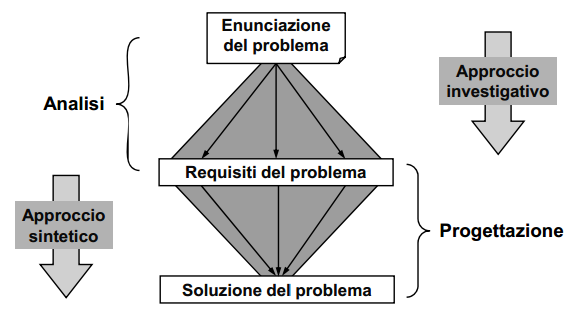
\includegraphics[width=0.75\columnwidth]{img1} % Example image
\end{center}

C'� un'apertura molto grande fatta per frazionamento (\textit{approccio investigativo}}) tipico dell'analista. Tutto non � necessariamente esplicito. Il lavoro del progettista � l'esatto opposto, deve riportare a sintesi i requisiti spezzettati e proporre una delle possibili soluzioni al problema, argomentando il valore di quella soluzione. Si torna da un punto singolare ad un punto singolare. L'analista ha fatto un buon lavoro se i requisiti sono tutti \textbf{tracciabili} e \textbf{verificabili}.\\
Dijkstra afferma che il compito che sta a un progettista di fare in modo che soddisfi i nostri bisogni � fatto di due parti:

\begin{itemize}

	\item \textbf{Stabilire le propriet�} di quella cosa in virt� delle quali soddisfo le propriet� attese e i bisogni. Questo � il compito dell'analista.
	\item \textbf{Fare quella cosa} in modo tale che le propriet� attese ci siano. E' quello che fa il progettista.

\end{itemize}

Uno dei compiti che aiuta il progettista � \textbf{fissare un'architettura}, cio� il modo in cui affrontiamo la struttura della soluzione. Ci sono diversi punti di vista che devono avere tutti la stessa soluzione:

\begin{itemize}

	\item \textbf{Committente}, che ha la visione del prodotto;
	\item \textbf{Fornitore}, confini del lavoro commissionato;
	\item \textbf{Analista}, che fissa vincoli e rischi tecnologici;
	\item \textbf{Progettista} che ha il compito di portare alla sintesi;
	\item \textbf{Architetto}

\end{itemize}

Un progettista che lavora strettamente sul progetto fa \textbf{scelte tattiche} sul breve periodo, mentre un architetto ha \textbf{governance}, ha una visione sul lungo periodo. Vogliamo che il progettista si avvicini il pi� possibile all'architetto. \textbf{Architettura come un mezzo} per raggiungere un fine. L'architettura ha una soluzione che � costruttiva e si pu� fare, � fatta di scelte costruttive che si amalgamano molto bene insieme. ``\textit{L'arte � un fine, l'architettura un mezzo}'' (Wells). Prima della fine degli anni '80 l'architettura veniva. L applicata solamente al sistema fisico. La nozione di architettura software appare per la prima volta nel 1992. Architettura sw fatta di:

\begin{itemize}

	\item \textbf{Elementi costruttivi};
	\item \textbf{Forma di queste parti};
	\item \textbf{Rational}, con una giustificazione.

\end{itemize}

Dobbiamo cercare queste tre cose. Architettura sw come insieme di \textbf{componenti}, \textbf{connessioni} e \textbf{vincoli}.

\begin{itemize}

	\item Un insieme di espressioni di bisogni che vengono dagli stakeholder (requisiti);
	\item Una spiegazione esplicita che giustifica le scelte e che sia razionale.

\end{itemize}

Prima di avere componenti, connessioni e vincoli bisogna avere l'idea di come sono le parti, dobbiamo avere un principio costruttivo. Sapere che forma devono avere le parti per ottenere le caratteristiche che mi servono. Esponendo un'interfaccia mostro che cosa offro. Ogni architettura ha uno \textbf{stile} architetturale riconoscibile. Secondo ISO/IEC/IEEE 42010-2011:

\begin{itemize}

	\item L'architettura � un modo per distinguere le parti (\textit{divide});
	\item Quelle parti sono organizzate (\textit{impera});
	\item Per poter avere un'organizzazione di parti bisogna avere delle interfacce che facilitino l'organizzazione;
	\item Paradigma di composizione, il criterio con cui metto insieme queste parti, regole, criteri, vincoli che hanno impatto sulla manutenzione futura.

\end{itemize}

Assunto di aver capito  questo, cerchiamo quali sono le qualit� da perseguire in un'architettura:

\begin{itemize}

	\item

\end{itemize}}

\end{document}